

\documentclass{standalone}
\usepackage{tikz}
\usetikzlibrary{shapes.geometric, arrows}

\begin{document}

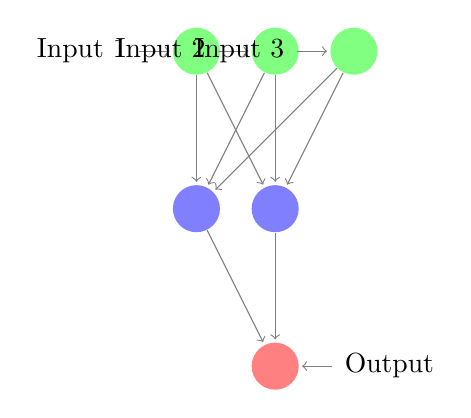
\begin{tikzpicture}[shorten >=1pt,->,draw=black!50, node distance=2.5cm]
    \tikzstyle{every pin edge}=[<-,shorten <=1pt]
    \tikzstyle{neuron}=[circle,fill=black!25,minimum size=17pt,inner sep=0pt]
    \tikzstyle{input neuron}=[neuron, fill=green!50];
    \tikzstyle{output neuron}=[neuron, fill=red!50];
    \tikzstyle{hidden neuron}=[neuron, fill=blue!50];
    
    % Draw the input layer nodes
    \foreach \name / \x in {1/1, 2/2, 3/3}
        \node[input neuron, pin=left:Input \x] (I-\name) at (\x, 0) {};
    
    % Draw the hidden layer nodes
    \foreach \name / \x in {1/1, 2/2}
        \node[hidden neuron] (H-\name) at (\x, -2) {};
        
    % Draw the output layer node
    \node[output neuron, pin=right:Output] (O) at (2,-4) {};
    
    % Connect every node in the input layer with every node in the hidden layer
    \foreach \source in {1,2,3}
        \foreach \dest in {1,2}
            \path (I-\source) edge (H-\dest);
            
    % Connect every node in the hidden layer with the output layer
    \foreach \source in {1,2}
        \path (H-\source) edge (O);

\end{tikzpicture}
\end{document}
